%%%%%%%%%%%%%%%%%%%%%
%								%
%	ESTADO DEL ARTE				%
%								%
%%%%%%%%%%%%%%%%%%%%%
\chapter{Estado del Arte}\label{cap:estadoArte}



%Por definición \textit{e-Commerce}: Transacción comercial electrónica, así como sobre Internet.
%
%Vender y realizar transacciones como estas se pueden hacer gracias a \textit{World Wide Web}, el cual es una convinación global de \textit{links}, información, paginas \textit{web} y \textit{e-Commerce websites}.
%
%Con el fin de considerar 

\section{\ecommerce}

\subsection{Categorías de \ecommerce}

Tecnología digital avanzada, combinada con las empresas y los clientes de estas tecnologías, impulsan \ecommerce. De igual forma que las tecnologías digitales, \ecommerce no pudo alcanzar su meta en un movimiento. En cuanto a las empresas y clientes, \ecommerce de diferentes tipos y niveles implica diferentes oportunidades \cite{zheng2009fundamentals}.

En relación a categorías de transacciones, \ecommerce se divide en 5 tipos:
\begin{figure}[h!]
	\centering
	\includegraphics[width=0.5\textwidth]{figuras/ecommerce_types.png}
	\caption{Categorias de \ecommerce.}
\end{figure}

\begin{itemize}
	\item \textbf{\btob}. Es simplemente definido como \ecommerce entre compañías. Este es el tipo de \ecommerce que tiene que ver con las relaciones entre y dentro de los negocios. Cerca del 80\% de \ecommerce que existe, corresponde a esta categoría, y cada vez son mas los expertos que predicen que \btob \ecommerce continuara su crecimiento a una velocidad mayor que el segmento \btoc.

%B2B e-commerce is simply defined as e-commerce between companies. This is the type of e-commerce that deals with relationships between and among businesses. About 80\% of e-commerce is of this type, and most experts predict that B2B ecommerce will continue to grow faster than the B2C segment.

	\item \textbf{\btoc}. En este caso, \internet es utilizado por negocios y empresas para proveer bienes y servicios por sities \webINT a los clientes. Actualmente varios tipos de sitios \webINT \btoc están repartidos por \internet para suministrar a los clientes una variedad de bienes y servicios que van desde flores y libros, hasta los ordenadores y autos, etc.

	\item \textbf{\btog}.El gobierno, como administrador nacional, desempeña un papel importante en la orientación, administración y ajuste de la economía. El advenimiento de la era de \ecommerce planteó fundamentos \ecommerce las nuevas solicitudes de las funciones originales de los gobiernos. Por un lado, el gobierno debería  administrar \emarket efectivamente y prestar un mejor servicio a las empresas y al público a través de \egoverment. Por otra parte, los gobiernos, como los \textit{"grandes clientes"} en economía deberían tomar la iniciativa para adoptar \ecommerce y ofrecer maneras eficientes a través de invitación de licitación electrónica para las contrataciones públicas.

%Governments, as national administrators, play a significant role in guiding, administrating and adjusting economy. The advent of e-commerce age put forward Fundamentals of E-commerce the new request to the original functions of governments. Governments should administrate e-market effectively and render better service to enterprises and the public by e-government on the one hand. Governments, as the “big clients” in economy should take the lead to adopt e-commerce and offer efficient path through electronic tender invitation for government procurement on the other hand.

	%TODO
	\item \textbf{\gtog}.

	\item \textbf{\ctoc}. Es un comercio simple entre individuos privados o consumidores. Este tipo de \ecommerce es caracterizado por el crecimiento de mercados electrónicos y las subastas \online, particularmente en industrias verticales donde empresas/negocios pueden pujar por lo que quieren de entre varios proveedores.
%Consumer-to-consumer e-commerce or C2C is simply commerce between private individuals or consumers. This type of e-commerce is characterized by the growth of electronic marketplaces and online auctions, particularly in vertical industries where firms/businesses can bid for what they want from among multiple suppliers.

	%TODO
	\item \textbf{\mcommerce}.
	
\end{itemize}

\subsection{\keyelements de un sitio \ecommerce \cite{inbook_ecommerce_keyelements}}

%TODO
\subsubsection{Domain y Hosting}

\subsubsection{Diseño}
El diseño del sitio es el principal elemento en determinar si el visitante se queda o se va.

%TODO
\subsubsection{\usabilityQA}

%TODO
\subsubsection{conversion}

%TODO
\subsubsection{\checkoutCOM}

%TODO
\subsubsection{Taking Payments}

%TODO
\subsubsection{Product Pages}

%TODO
\subsubsection{On-Site SEO (Search Engine Optimization)}

%TODO
\subsubsection{Content Management System \& Automation}

%TODO
\subsubsection{Key \ecommerce Features}

%TODO
\subsubsection{Operation \& Order Management}

%TODO
\subsubsection{Information Pages}


\subsubsection{\security, \trust \& Testimonials}

\trust y \familiarity influencian \ecommerce, como insinúa \luhmanntheory. Especialmente los datos muestran que tanto \trust en un \consumer \internet y \familiarity con el \seller y sus procedimientos influencian dos aspectos distintos de \ecommerce en sitios de venta de libros: \inquiry y \purchase. La influencia de la  \familiarity y \trust son especialmente fuertes en intenciones  de las personas para \purchase. Segundo, los datos muestran que \trust y \familiarity son claramente diferentes construcciones, y la \trust es significativamente afectada por \familiarity, y no solo por la social disposición de la gente para \trust. El modelo de investigación muestra que  \ecommerce puede ser evaluado en el contexto de un ambiente social complejo basado en \luhmanntheory. Bajo tales circunstancias, tanto \trust como \familiarity influencian intenciones de comportamiento\cite{gefen2000commerce}.

\security influencia \trust. Por ejemplo, en el caso de \amazon, una persona \familiarity con el concepto de \secureintcom podría permitir que se entreguen creencias específicas relativas a la medida de seguridad que ellos esperan del vendedor (\trust)\cite{gefen2000commerce}.

\ebay realizo un estudio en donde demostró que la reputación \ecommerce de un \seller es un determinante, aunque no un determinante principal, del precio que los \sellers recibían en sus subastas. En ausencia de otros, recursos mas directos de información del \itemsCommerce, un \consumer en \internet debe confiar en la precisión de la descripción del \itemsCommerce del \sellers y la confiabilidad de la entrega del \itemsCommerce del \sellers para decidir si, y cuanto esta dispuesto a ofertar por el bien. Dicho de otra manera, la reputación del \sellers se convierte en una consideración en la voluntad del \consumer para hacer una oferta en el artículo de la subasta. El resultado empírico muestra que un \seller con una mejor reputación puede esperar recibir ofertas superiores para sus \itemsCommerce subastados. Sin embargo, aunque la reputación es una determinante estadisticamente significativa, su impacto tiende a ser pequeño\cite{melnik2002does}.

En este sentido, los nuevos \seller de subasta en el \websites pueden considerar difícil competir con los \sellers existentes quienes tienen establecida una reputación positiva. Además, en la ausencia de un mecanismo que permitan que los \ratings sean transferidos entre sitios, un \seller quien ya tiene un alto \rating en un \websiteINT de subastas \online puede enfrentar un costo en cambiar a otro \websiteINT de subastas \online. \textit{Reputación} obviamente provee algunos beneficios para los \consumers buscando la \internet por \itemsCommerce para los cuales realizar una oferta. Sin embargo, tal \textit{reputación} puede también implicar algunos costos a los \consumers, si el desarrollo de reputación para subastas \online actúa como barrera de entrada para nuevos \websites de  subastas \online  y da poder de monopolio a los \websites de subastas \online ya establecidos\cite{melnik2002does}.

%TODO
\subsubsection{Marketing Elements}

%TODO
\subsubsection{Analytics/reports}





Aunque no es relevante para el \frameworkPC, es importante destacar la importancia que tiene este tópico en el éxito que pueda tener una solución \ecommerce. 

%TODO

\openSourcePC \ecommerce \shoppingCarts ofrecen muchas ventajas para \textit{small businesses}. Soluciones \openSourcePC pueden ser desarrolladas para ajustarse a las necesidades del negociante. Ellos contienen una gran combinación de características a un mínimo costo. Y, aunque las opciones de soporte pueden ser mas limitadas que las propietarias o \textit{hosted platforms}, soluciones independientes \openSourcePC generalmente tienen grandes comunidades de desarrolladores y socios para ayudar a los nuevos comerciantes.

\section{Ejemplos de \frameworksPC \ecommerce existentes}

Aquí hay una lista de 11 soluciones \ecommerce \openSourcePC. El \coreAS de todas las aplicaciones es \free. Cada aplicación tiene extensiones \free y \premium, y opciones de soporte para mejorar el desarrollo de la \store.

\begin{itemize}
	\item \textbf{\nameOpenCart}. Es una aplicación \openSourcePC, basada en \phpNAME, es una solución \ecommerce para comerciantes \online. \nameOpenCart tiene una comunidad activa y leal para el apoyo de usuarios, así como una lista de socios comerciales para instalación y customización profesional. En \nameOpenCart existen mas de 20 medios de pago, y mas de 8 métodos de envío para la descarga por defecto, con cientos de métodos adicionales para el envío y el pago en su directorio de extensiones. \nameOpenCart también fue diseñado para un manejo sencillo de múltiples compras desde una interfaz de administración. Tiene más de 2700 \themes.
	
	\begin{figure}[H]
		\centering
		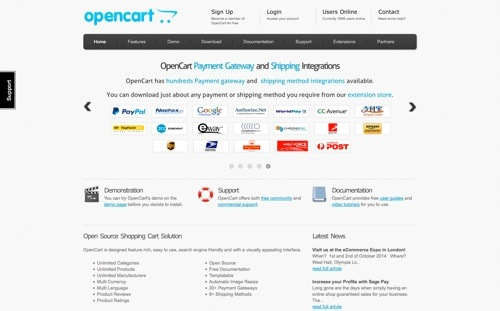
\includegraphics[width=0.5\textwidth]{figuras/cap1/openCartWebsite.jpg}
		\caption{\nameOpenCart \websiteINT \cite{online_OpenCartWebsite}.}
	\end{figure}


	\item \textbf{\namePrestaShop}. Es una solución \ecommerce \openSourcePC, escrita en \phpNAME y basada en \smartyTemplateEngine. \namePrestaShop viene con mas de 310 características integradas y 3500 módulos y \templates. Cuenta con ventas cruzadas, productos descargables, la exportación de productos, una pagina de pago, envió, descuentos y mucho mas. Descargado mas de 4 millones de veces, \namePrestaShop es usado en 160 países y traducido a 63 idiomas. Tiene mas de 600000 miembros en su comunidad.

	\begin{figure}[H]
		\centering
		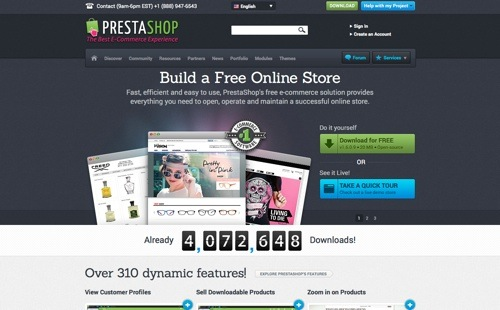
\includegraphics[width=0.5\textwidth]{figuras/cap1/PrestaShopWebsite.jpg}
		\caption{\namePrestaShop \websiteINT \cite{online_PrestaShop}.}
	\end{figure}


	\item \textbf{\nameMagento \Community \Edition} es una version \free y \openSourcePC de  una plataforma \ecommerce. Los comerciantes pueden acceder a características adicionales instalando las extensiones desde el gran \nameMagento \connectCustom \marketplace. No existe soporte para \nameMagento \Community \Edition, así que las respuestas a las preguntas técnicas deben ser resultas a través del foro de usuarios. Un detalle, \nameMagento ha anunciado el cierro de su \hosted \solution, \nameMagento \go, por ahora no habrían problemas con \Community \Edition. \nameMagento \Community \Edition soporta mas de 200000 sitios de clientes .

	\begin{figure}[H]
		\centering
		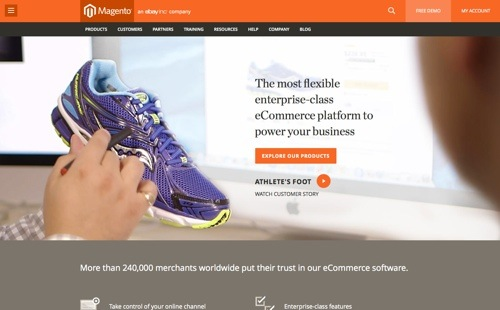
\includegraphics[width=0.5\textwidth]{figuras/cap1/MagentoWebsite.jpg}
		\caption{\nameMagento \websiteINT \cite{online_Magento}.}
	\end{figure}


	\item \textbf{\nameZenCart} es una aplicación \ecommerce \openSourcePC escrita en \phpNAME.\nameZenCart \branched desde el código \nameOsCommerce en 2003, con una solución que era mas \templateBased. Tiene mas de 1800 \addOns en 16 categorías. La comunidad de apoyo de \nameZenCart tiene aproximadamente 150000 miembros y 200000 \threadsPL.

	\begin{figure}[H]
		\centering
		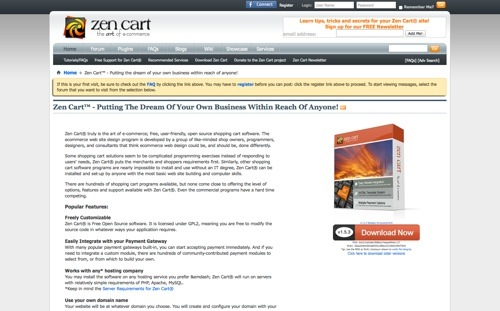
\includegraphics[width=0.5\textwidth]{figuras/cap1/ZenCartWebsite.jpg}
		\caption{\nameZenCart \websiteINT \cite{online_ZenCart}.}
	\end{figure}


	\item \textbf{\nameSpreeCommerce} es una solución \ecommerce \openSourcePC  basado en \rubyonrailsNAME. La plataforma modular permite configurar, complementar, o reemplazar cualquier funcionalidad que necesites. \nameSpreeCommerce tiene mas de 45000 tiendas la plataforma al rededor del mundo, incluyendo \chipotle \cite{online_Chipotle}. \nameSpreeCommerce ha sido traducido a más de 30 idiomas.

	\begin{figure}[H]
		\centering
		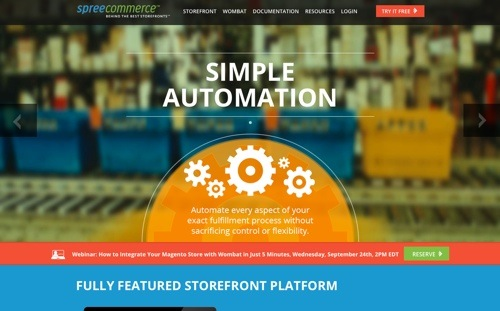
\includegraphics[width=0.5\textwidth]{figuras/cap1/SpreeCommerceWebsite.jpg}
		\caption{\nameSpreeCommerce \websiteINT \cite{online_SpreeCommerce}.}
	\end{figure}

	\item \textbf{\nameDrupalCommerce} es una aplicación \ecommerce desarrollado por \commerceGuys. Construido sobre \drupalContManSys. \nameDrupalCommerce ofrece un sistema de administración de producto completo, carro de compra varios lenguajes y monedas; y forma de pago. La lista de extension de \nameDrupalCommerce es una integración completamente en\thirdParty para formas de pago,servicios de cumplimiento, aplicaciones de contabilidad, redes sociales y mucho mas. Paquetes de soporte técnico están disponibles por \commerceGuys.

	\begin{figure}[H]
		\centering
		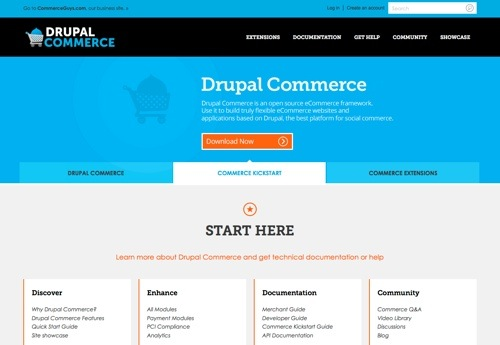
\includegraphics[width=0.5\textwidth]{figuras/cap1/DrupalCommerceWebsite.jpg}
		\caption{\nameDrupalCommerce \websiteINT \cite{online_DrupalCommerce}.}
	\end{figure}

	\item \textbf{\nameOsCommerce} (i.e., \openSourcePC \commerce)es uno de las primeras aplicaciones \ecommerce \openSourcePC. Más de 7000 \free \addOns han sido subidos por su comunidad para customizar una \store \online. \nameOsCommerce es usado por cerca de 13000 sitios registrados. La comunidad de apoyo tiene aproximadamente 280000 miembros los cuales han contribuido con 1.5 millones de \posts en los foros. La comunidad directa juntos con miembros de otra comunidad están disponibles en vivo en el \chat \room.

	\begin{figure}[H]
		\centering
		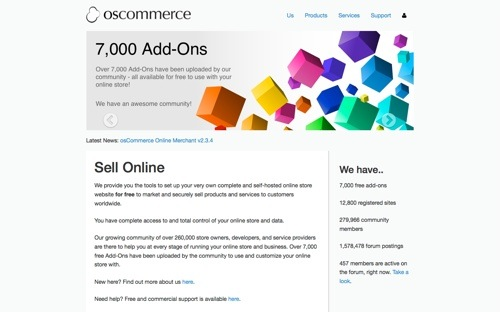
\includegraphics[width=0.5\textwidth]{figuras/cap1/osCommerceWebsite.jpg}
		\caption{\nameOsCommerce \websiteINT \cite{online_osCommerce}.}
	\end{figure}

	\item \textbf{\nameSimpleCart} es un \free y \openSourcePC \javaScriptNAME \shoppingCart. Con su pequeño tamaño, \nameSimpleCart esta diseñado para mantener simple  y sitios con alto tráfico \running \fast. \nameSimpleCart tienen la habilidad de pagar con \paypalCheckout, \googleCheckout, y \amazonPayments. \email \checkoutCOM e integración con \AuthorizeNet llegarán pronto.
	
	\begin{figure}[H]
		\centering
		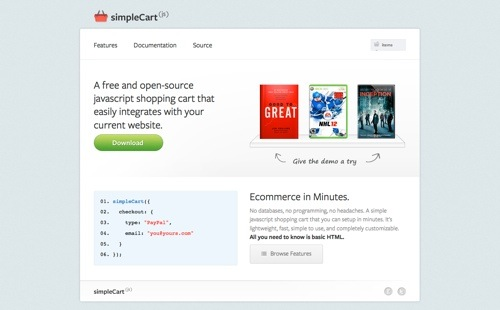
\includegraphics[width=0.5\textwidth]{figuras/cap1/simpleCartWebsite.jpg}
		\caption{\nameSimpleCart \websiteINT \cite{online_simpleCart}.}
	\end{figure}

	\item \textbf{\nameWooCommerce} es una aplicación \ecommerce \free \openSourcePC que permite a los comerciantes transformar \wordPress \sites en \stores. \nameWooCommerce fue desarrollado por \wooThemes desde un \fork de \nameJigoshop. \nameWooCommerce tiene una larga variedad de  \plugins y  \themes de \wooThemes, como de sitios \thirdParty tales como \themeForest \cite{online_ThemeForest} y \codeCanyon \cite{online_CodeCanyon}. Con cerca de 4.5 millones de descargas desde \wordPressOrg\cite{online_WordPress}, \nameWooCommerce es una solución \ecommerce muy popular para \wordPress. Para obtener el soporte oficial de \wooThemes, es necesario comprar un producto. De otra manera, obtener ayuda desde la comunidad activa del foro.

	\begin{figure}[H]
		\centering
		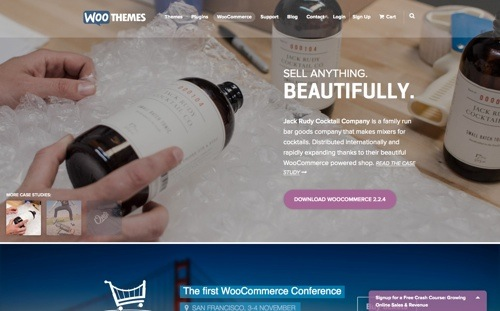
\includegraphics[width=0.5\textwidth]{figuras/cap1/WooCommerceWebsite.jpg}
		\caption{\nameWooCommerce \websiteINT \cite{online_WooCommerce}.}
	\end{figure}

	\item \textbf{\nameWPECommerce} es otra aplicación popular obtenida desde la conversión del  sitio \wordPress a una \ecommerce \store.\nameWPECommerce tiene cerca de 3 millones de descarga de \plugin desde \wordPressOrg\cite{online_WordPress}. Usa el propio \htmlNAME y \cssNAME y obtén el control completo sobre la vista y la experiencia de tu \online \store. \nameWPECommerce tiene una gran variedad de características estándar, incluyendo \multiTierPricing para descuentos por cantidad e integración con redes sociales para \marketing. Para soporte, hay tutoriales en video y un foro en \wordPressOrg, también como consultantes de características para ayuda profesional.

	\begin{figure}[H]
		\centering
		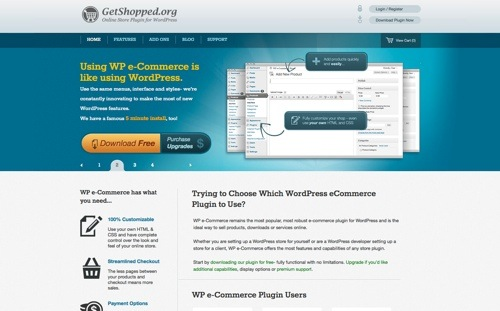
\includegraphics[width=0.5\textwidth]{figuras/cap1/WPECommerceWebsite.jpg}
		\caption{\nameWPECommerce \websiteINT \cite{online_WPECommerce}.}
	\end{figure}

	\item \textbf{\nameJigoshop} es una solución \ecommerce \free y \openSourcePC basado en \wordPress. Liberado en 2011, \nameJigoshop es el predecesor para \nameWooCommerce. \nameJigoshop tiene mas de 30 \themes, 100 extensiones, y tres \theme \frameworksPC. \nameJigoshop es \free, así como el soporte a \wordPressOrg. Sin embargo, el acceso a la comunidad de \nameJigoshop comienza desde \$40 por mes.

	\begin{figure}[H]
		\centering
		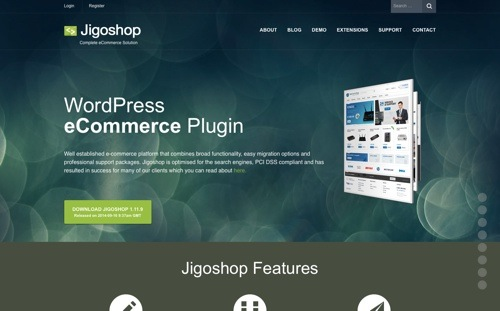
\includegraphics[width=0.5\textwidth]{figuras/cap1/JigoshopWebsite.jpg}
		\caption{\nameJigoshop \textit{website}\cite{online_Jigoshop}.}
	\end{figure}

\end{itemize}


\subsection{Resumen de \frameworksPC disponibles}
%%%%%%%%%%%%%%%%%%%%%%%%%%%%%%%%%%%%%%%%%%%%%%%%%%%%%%%%%%%%%%%%%%%%%%%%%%%%%
%%%%%%%%%%%%%%%%%%%		     RESUMEN GENERAL	   	%%%%%%%%%%%%%%%%%%%%%%%%%
%%%%%%%%%%%%%%%%%%%%%%%%%%%%%%%%%%%%%%%%%%%%%%%%%%%%%%%%%%%%%%%%%%%%%%%%%%%%%
\subsubsection{Resumen general de los \frameworksPC disponibles}

En \reftabla{tab:resume_technology_ecommerce} hay un resumen de información básica general sobre \shoppingCarts.
%Basic general information about the shopping carts including creator, software license and framework, and updates.

\begin{table}[H]
    \tiny
    \centering
%\begin{tabular}{ |C{0.3\paperwidth}|C{0.3\paperwidth}| }
\begin{tabular}{ |l|c|c|c|c|c| }

\hline
	&
	\freePC \dataBaseDB \backendAS support&
	Language&
	\wafAS&
	\License&
	version

\\ \hline
	\nameOpenCart &
	\mysqlNAME&
	\phpNAME&
	&
	\gplthreelicense &
	2.0.1.1
	
\\ \hline
	\namePrestaShop &
	\mysqlNAME&
	\phpNAME&
	&
	\opslicense &
	1.6.0.11
	
\\ \hline
	\nameMagento &
	\mysqlNAME&
	\phpNAME&
	\zendNAME \cite{online_zend_framework}&
	\opslicense &
	1.9.1.0
	
\\ \hline
	\nameZenCart &
	\mysqlNAME&
	\phpNAME&
	&
	\gpllicense &
	1.5.4
 
\\ \hline
	\nameSpreeCommerce &
	\mysqlNAME, \postgresql, \sqlitethree&
	\rubyNAME \cite{online_ruby_language}&
	\rubyonrailsNAME \cite{online_ruby_rails}&
	\bsdthreelicense&
	2.2.2

\\ \hline
	\nameDrupalCommerce &
	\mysqlNAME, \postgresql, \sqlitethree&
	\phpNAME&
	\drupalNAME \cite{online_drupal}&
	\gpllicense &
	1.10
	
\\ \hline
	\nameOsCommerce &
	\mysqlNAME&
	\phpNAME&
	&
	\gpllicense &
	2.3.4

\\ \hline
	\nameSimpleCart &
	&
	&
	&
	&
	
\\ \hline
	\nameWooCommerce &
	\mysqlNAME&
	\phpNAME&
	\wordPressNAME \cite{online_wordpress}&
	\gpllicense &
	2.2.7
	
\\ \hline
	\nameWPECommerce &
	&
	&
	&
	&
	
\\ \hline
	\nameJigoshop &
	\mysqlNAME&
	\phpNAME&
	\wordPressNAME \cite{online_wordpress}&
	\gpllicense &
	1.12.3
	
\\ \hline
\end{tabular}
    \caption{ Resumen general de los \frameworksPC disponibles}
    \label{tab:resume_technology_ecommerce}
\end{table}



%
%\begin{table}[h!]
%    \tiny
%    \centering
%%\begin{tabular}{ |C{0.3\paperwidth}|C{0.3\paperwidth}| }
%\begin{tabular}{ |l|c|c|c|c|c|c| }
%\hline
%	&
%	traider\cite{online_Traider}&
%	ReactionCommerce\cite{online_reactionCommerce}&
%	NodeShop\cite{online_NodeShop}&
%	Forward\cite{online_Forward}&
%	Ottemo \cite{online_framework_ottemo_officialsite}&
%	ZRECommerce \cite{online_framework_zrecommerce_officialsite}
% 
%\\ \hline
%	Tecnología &
%	bootstrap, nodejs and mongodb &
%	Nodejs, Meteor, Mongodb, CoffeScript, Bootstrap, Docker&
%	&
%	
%
%\\ \hline
%	Mobile &
%	&
%	&
%	&
%\\ \hline
%	version &
%	&
%	&
%	0.06 ( 21/08/2013 )&
%	0.1
%
%\\ \hline
%\end{tabular}
%    \caption{ Resumen tecnologías entre diferentes opciones \textit{e-Commerce}}
%    \label{tab:resume_technology_ecommerce2}
%\end{table}


%%%%%%%%%%%%%%%%%%%%%%%%%%%%%%%%%%%%%%%%%%%%%%%%%%%%%%%%%%%%%%%%%%%%%%%%%%%%%
%%%%%%%%%%%%%%%%%%%		  CUSTOMERS FEATURES		%%%%%%%%%%%%%%%%%%%%%%%%%
%%%%%%%%%%%%%%%%%%%%%%%%%%%%%%%%%%%%%%%%%%%%%%%%%%%%%%%%%%%%%%%%%%%%%%%%%%%%%

\begin{table}[H]
    \tiny
    \centering
%\begin{tabular}{ |C{0.3\paperwidth}|C{0.3\paperwidth}| }
\begin{tabular}{ |l|c|c|c|c|c|c|c| }

\hline
	&
	Buscar&
	Imagen \itemCOM&
	\raiting \itemCOM&
	\review \itemCOM&
	\wishlist&
	\itemsCOM populares&
	Redes sociales

\\ \hline
	\nameOpenCart &
	&
	&
	&
	&
	&
	&
	
\\ \hline
	\namePrestaShop &
	\anwerYes&
	\anwerYes&
	\anwerYes&
	\anwerYes&
	\anwerYes&
	\anwerYes&
	\anwerYes
	
\\ \hline
	\nameMagento &
	\anwerYes&
	\anwerYes&
	\anwerYes&
	\anwerYes&
	\anwerYes&
	\anwerYes&
	\anwerYes
	
\\ \hline
	\nameZenCart &
	\anwerYes&
	\anwerYes&
	\anwerYes&
	\anwerYes&
	\freePC \addOn&
	\anwerYes&
	\freePC \addOn
 
\\ \hline
	\nameSpreeCommerce &
	&
	&
	&
	&
	&
	&

\\ \hline
	\nameDrupalCommerce &
	\anwerYes&
	\anwerYes&
	\anwerYes&
	\anwerYes&
	\anwerYes&
	\anwerYes&
	\anwerYes
	
\\ \hline
	\nameOsCommerce &
	\anwerYes&
	\anwerNo&
	\anwerYes&
	\anwerYes&
	\anwerNo&
	\anwerYes&
	\anwerYes

\\ \hline
	\nameSimpleCart &
	&
	&
	&
	&
	&
	&
	
\\ \hline
	\nameWooCommerce &
	&
	&
	&
	&
	&
	&
	
\\ \hline
	\nameWPECommerce &
	&
	&
	&
	&
	&
	&
	
\\ \hline
	\nameJigoshop &
	\anwerYes&
	\anwerYes&
	\anwerYes&
	\anwerYes&
	\anwerYes&
	\anwerYes&
	\anwerYes
	
\\ \hline
\end{tabular}
    \caption{ Características de \customers}
    \label{tab:customers_features_ecommerce}
\end{table}

%%%%%%%%%%%%%%%%%%%%%%%%%%%%%%%%%%%%%%%%%%%%%%%%%%%%%%%%%%%%%%%%%%%%%%%%%%%%%
%%%%%%%%%%%%%%%%%%%	  ADMINISTRATION AREA FEATURES	%%%%%%%%%%%%%%%%%%%%%%%%%
%%%%%%%%%%%%%%%%%%%%%%%%%%%%%%%%%%%%%%%%%%%%%%%%%%%%%%%%%%%%%%%%%%%%%%%%%%%%%

\subsubsection{Características de administración}

Información sobre las características que los \shoppingCarts ofrecen.

\begin{table}[h!]
    \tiny
	\centering
%\begin{tabular}{ |C{0.3\paperwidth}|C{0.3\paperwidth}| }
\begin{tabular}{ |l|c|c|c| }	

\hline
	&
	Estadísticas &
	Control de \stock &
	Editor \wysiwyg

\\ \hline
	\nameOpenCart &
	&
	&
	
\\ \hline
	\namePrestaShop &
	\anwerYes&
	\anwerYes&
	\anwerYes
	
\\ \hline
	\nameMagento&
	\anwerYes&
	\anwerYes&
	\anwerYes
	
\\ \hline
	\nameZenCart &
	\anwerYes&
	\anwerYes&
	\freePC \addOn
 
\\ \hline
	\nameSpreeCommerce &
	&
	&
	

\\ \hline
	\nameDrupalCommerce&
	\anwerYes&
	\anwerYes&
	\anwerYes
	
\\ \hline
	\nameOsCommerce &
	\anwerYes&
	\anwerYes&
	\freePC \addOn

\\ \hline
	\nameSimpleCart &
	&
	&
	
	
\\ \hline
	\nameWooCommerce &
	&
	&
	
	
\\ \hline
	\nameWPECommerce &
	&
	&
	
	
\\ \hline
	\nameJigoshop &
	\anwerYes&
	\anwerYes&
	\anwerYes
	
\\ \hline

\end{tabular}
    \caption{ Soporte de \checkoutCOM }
    \label{tab:administration_area_features}
\end{table}


%%%%%%%%%%%%%%%%%%%%%%%%%%%%%%%%%%%%%%%%%%%%%%%%%%%%%%%%%%%%%%%%%%%%%%%%%%%%%
%%%%%%%%%%%%%%%%%%%	  ADMINISTRATION AREA FEATURES	%%%%%%%%%%%%%%%%%%%%%%%%%
%%%%%%%%%%%%%%%%%%%%%%%%%%%%%%%%%%%%%%%%%%%%%%%%%%%%%%%%%%%%%%%%%%%%%%%%%%%%%

\subsubsection{Características de \rewards para \customers}

Información sobre las características que los \shoppingCarts ofrecen.

\begin{table}[h!]
    \tiny
	\centering
%\begin{tabular}{ |C{0.3\paperwidth}|C{0.3\paperwidth}| }
\begin{tabular}{ |l|c|c|c|c|c|c|c| }	

\hline
	&
	Cupones&
	Certificados de \gifts&
	Descuentos \membership&
	Categorías \membershipOnly&
	\itemCOM \membershipOnly&
	Puntos de \reward&
	Ofertas especiales

\\ \hline
	\nameOpenCart &
	&
	&
	&
	&
	&
	&
	
\\ \hline
	\namePrestaShop &
	\anwerYes&
	\anwerYes&
	\anwerYes&
	\anwerYes&
	\anwerYes&
	\anwerYes
	
\\ \hline
	\nameMagento&
	\anwerYes&
	\anwerYes&
	\anwerYes&
	\anwerYes&
	\thirdPartyModule&
	\anwerYes
	
\\ \hline
	\nameZenCart &
	\anwerYes&
	\anwerYes&
	\anwerYes&
	\anwerNo&
	\anwerNo&
	\anwerYes&
	\anwerYes
 
\\ \hline
	\nameSpreeCommerce &
	&
	&
	&
	&
	&
	&
	

\\ \hline
	\nameDrupalCommerce&
	\anwerYes&
	\anwerYes&
	\anwerYes&
	\anwerYes&
	\anwerYes&
	\anwerNo&
	\anwerYes
	
\\ \hline
	\nameOsCommerce &
	\anwerYes&
	\anwerYes&
	\freePC \addOn&
	&
	&

\\ \hline
	\nameSimpleCart &
	&
	&
	&
	&
	&
	&
	
	
\\ \hline
	\nameWooCommerce &
	&
	&
	&
	&
	&
	&
	
	
\\ \hline
	\nameWPECommerce &
	&
	&
	&
	&
	&
	&
	
\\ \hline
	\nameJigoshop &
	\anwerYes&
	\anwerYes&
	\anwerYes&
	\anwerYes&
	\anwerYes&
	\anwerYes&
	\anwerYes
	
\\ \hline

\end{tabular}
    \caption{ Características de \rewards para \customers }
    \label{tab:customer_reward_features}
\end{table}


%%%%%%%%%%%%%%%%%%%%%%%%%%%%%%%%%%%%%%%%%%%%%%%%%%%%%%%%%%%%%%%%%%%%%%%%%%%%%
%%%%%%%%%%%%%%%%%%%%%%%%%%%%  CHECKOUT SUPPORT  %%%%%%%%%%%%%%%%%%%%%%%%%%%%%
%%%%%%%%%%%%%%%%%%%%%%%%%%%%%%%%%%%%%%%%%%%%%%%%%%%%%%%%%%%%%%%%%%%%%%%%%%%%%

\subsubsection{Soporte de \checkoutCOM}

En \reftabla{tab:checkout_support} se encuentra disponible la información  sobre los \checkoutCOM disponibles.

\begin{table}[h!]
    \tiny
	\centering
%\begin{tabular}{ |C{0.3\paperwidth}|C{0.3\paperwidth}| }
\begin{tabular}{ |l|c|c|c| }	

\hline
	&
	\googleCheckout &
	\paypalCheckout &
	\amazonCheckout

\\ \hline
	\nameOpenCart &
	&
	&
	
\\ \hline
	\namePrestaShop &
	\anwerYes&
	\anwerYes&
	\anwerYes
	
\\ \hline
	\nameMagento&
	\anwerYes&
	\anwerYes&
	\freePC \addOn
	
\\ \hline
	\nameZenCart &
	\freePC \addOn&
	\anwerYes&
	\answerunknown
 
\\ \hline
	\nameSpreeCommerce &
	&
	&
	

\\ \hline
	\nameDrupalCommerce&
	\anwerYes&
	\anwerYes&
	\answerunknown
	
\\ \hline
	\nameOsCommerce &
	\anwerNo&
	\anwerNo&
	\answerunknown

\\ \hline
	\nameSimpleCart &
	&
	&
	
	
\\ \hline
	\nameWooCommerce &
	&
	&
	
	
\\ \hline
	\nameWPECommerce &
	&
	&
	
	
\\ \hline
	\nameJigoshop &
	\anwerYes&
	\anwerYes&
	\anwerYes
	
\\ \hline

\end{tabular}
    \caption{ Soporte de \checkoutCOM }
    \label{tab:checkout_support}
\end{table}


%%%%%%%%%%%%%%%%%%%%%%%%%%%%%%%%%%%%%%%%%%%%%%%%%%%%%%%%%%%%%%%%%%%%%%%%%%%%%%%
%%%%%%%%%%%%%%%%%%%	 	REAL TIME SHIPPING CALCULATION 		%%%%%%%%%%%%%%%%%%%
%%%%%%%%%%%%%%%%%%%%%%%%%%%%%%%%%%%%%%%%%%%%%%%%%%%%%%%%%%%%%%%%%%%%%%%%%%%%%%%

\subsubsection{Cálculo \shipping \realTimeINT}

Información sobre si \shoppingCarts tienen como característica cálculo \shipping \realTimeINT permite calcular cuanto tiempo costará enviar una orden in \realTimeINT cuando el cliente \checkoutCOM una orden.
%Information about if the Shopping Carts have Real Time Shipping Calculation built in to be able to calculate how much it will cost to ship an order in real time when the customer checks out an order.
\begin{table}[H]
    \tiny
   \centering
%\begin{tabular}{ |C{0.3\paperwidth}|C{0.3\paperwidth}| }
\begin{tabular}{ |l|c|c|c| }

\hline
	&
	\dhlName &
	\fedExName &
	\upsName

\\ \hline
	\nameOpenCart &
	&
	&
	
	
\\ \hline
	\namePrestaShop &
	\anwerNo&
	\anwerYes&
	\anwerYes
	
\\ \hline
	\nameMagento&
	\anwerYes&
	\anwerYes&
	\anwerYes
	
\\ \hline
	\nameZenCart &
	\freePC \addOn&
	\freePC \addOn&
	\anwerYes
 
\\ \hline
	\nameSpreeCommerce &
	&
	&

\\ \hline
	\nameDrupalCommerce&
	&
	&
	
\\ \hline
	\nameOsCommerce &
	\anwerNo&
	\anwerNo&
	\anwerNo

\\ \hline
	\nameSimpleCart &
	&
	&
	
\\ \hline
	\nameWooCommerce &
	&
	&
	
\\ \hline
	\nameWPECommerce &
	&
	&
	
\\ \hline
	\nameJigoshop &
	\anwerYes&
	\anwerYes&
	\anwerYes
	
\\ \hline

\end{tabular}
    \caption{Cálculo \shipping \realTimeINT}
    \label{tab:general_features_ecommerce}
\end{table}


%%%%%%%%%%%%%%%%%%%%%%%%%%%%%%%%%%%%%%%%%%%%%%%%%%%%%%%%%%%%%%%%%%%%%%%%%%%%%%%
%%%%%%%%%%%%%%%%%%%	  	Shipment tracking integration 		%%%%%%%%%%%%%%%%%%%
%%%%%%%%%%%%%%%%%%%%%%%%%%%%%%%%%%%%%%%%%%%%%%%%%%%%%%%%%%%%%%%%%%%%%%%%%%%%%%%

\subsubsection{Integración \tracking \shipping}

Información sobre si \shoppingCarts tienen integración de \tracking \shipping para mostrar a los \customers información de \tracking en la página de ordenes.
%Information about if the Shopping Carts have Shipment Tracking Integration to show the customers the tracking information on the View Order pages.
\begin{table}[H]
    \tiny
	\centering
%\begin{tabular}{ |C{0.3\paperwidth}|C{0.3\paperwidth}| }
\begin{tabular}{ |l|c|c|c| }

\hline
	&
	\dhlName &
	\fedExName &
	\upsName

\\ \hline
	\nameOpenCart &
	&
	&
	
\\ \hline	
	\namePrestaShop &
	\anwerNo&
	\anwerYes&
	\anwerYes
	
\\ \hline
	\nameMagento&
	\anwerYes&
	\anwerYes&
	\anwerYes
	
\\ \hline
	\nameZenCart &
	\freePC \addOn&
	\freePC \addOn&
	\freePC \addOn
 
\\ \hline
	\nameSpreeCommerce &
	&
	&

\\ \hline
	\nameDrupalCommerce&
	&
	&
	
\\ \hline
	\nameOsCommerce &
	\anwerNo&
	\anwerNo&
	\anwerNo

\\ \hline
	\nameSimpleCart &
	&
	&
	
\\ \hline
	\nameWooCommerce &
	&
	&
	
\\ \hline
	\nameWPECommerce &
	&
	&
	
\\ \hline
	\nameJigoshop &
	\anwerYes&
	\anwerYes&
	\anwerYes
	
\\ \hline
\end{tabular}
    \caption{Integración \tracking \shipping}
    \label{tab:Shipment_tracking_integration}
\end{table}



\section{Tecnologías }\label{cap:estadoArte:tecnologias}
%TODO agregar algo decente en este lugar.
A continuación se describen un conjunto de tecnologías que son agrupadas lógicamente de acuerdo a su función en el desarrollo de aplicaciones \webINT.

Estas tecnologías tienen en común que son herramientas que se ocupan en la actualidad además de tener la característica de ser \openSourcePC. 

\subsection{Bases de datos}

\begin{itemize}
	\item \textbf{\mongodbNAME} (de "hu\textbf{mongo}us") es un base de datos \documentOriented \openSourcePC, escrita en \cPlusPlus \cite{technology_mongodb}. \mongodbNAME evita las estructuras de \dataBaseDB tradicionales \tableBasedDB en favor de \documentsDB \jsonLikeCPT con \schemasDB dinámicos (\mongodbNAME llama al formato \bsonNAME), haciendo la integración de \dataPC en cierto tipo de aplicaciones mas fácil y rápido. \mongodbNAME es la \nosqlNAME líder, y la alcanzando una popularidad que supera a \postgresql \cite{online_db_engines_ranking}.
	%MongoDB (from humongous) is a cross-platform document-oriented database. Classified as a NoSQL database, MongoDB eschews the traditional table-based relational database structure in favor of JSON-like documents with dynamic schemas (MongoDB calls the format BSON), making the integration of data in certain types of applications easier and faster. [http://en.wikipedia.org/wiki/MongoDB]
	
	\item \textbf{\mysqlNAME} es una \rdbms \openSourcePC que se posiciona como la  segundo más utilizado a nivel mundial \cite{online_db_engines_ranking}\cite{online_dispelling_myths}. \mysqlNAME es una opción popular de \dataBaseDB para aplicaciones \webINT ampliamente utilizado en el \stackAS \lampNAME (y otros \stacksAS  \ampNAME).
	%MySQL is a popular choice of database for use in web applications, and is a central component of the widely used LAMP open source web application software stack (and other 'AMP' stacks). LAMP is an acronym for "Linux, Apache, MySQL, Perl/PHP/Python." Free-software-open source projects that require a full-featured database management system often use MySQL.
	
	\item \textbf{\postgresql} es una \ordbms con énfasis en \extensibilityQA y normas de cumplimiento. Como \serverAS de \dataBaseDB, su primera función es \store \dataPC, de forma segura y apoyar las mejores prácticas, y recuperarlo más tarde, a petición de otras aplicaciones de \softwarePC, ya sea que estén \running en el mismo computador o \running en otro computador a través  de una \network (incluido \internet). Puede manejar las cargas de trabajo que van desde pequeñas aplicaciones de una sola máquina a grandes aplicaciones orientados a \internet con muchos usuarios concurrentes.
	% (ORDBMS) with an emphasis on extensibility and standards-compliance. As a database server, its primary function is to store data, securely and supporting best practices, and retrieve it later, as requested by other software applications, be it those on the same computer or those running on another computer across a network (including the Internet). It can handle workloads ranging from small single-machine applications to large Internet-facing applications with many concurrent users. Recent versions also provide replication of the database itself for availability and scalability.
	
	\item \textbf{\sqlite} es una \rdbms contenida en una librería \cprogramming. A diferencia de otras \dbmangesystem, \sqlite no esta implementado como un proceso independiente del \clientAS. En contraste, es parte del programa en uso \cite{online_video_introduction_sqlite}.
	%is a relational database management system contained in a C programming library. In contrast to other database management systems, SQLite is not implemented as a separate process that a client program running in another process accesses. Rather, it is part of the using program.
	
	\item \textbf{\cassandraNAME} es un \nosqlNAME \wideColumnDB \store \openSourcePC diseñado para manejar gran cantidad de \dataPC sobre muchos \commodityServerPC, proporcionando \highAvailabilityDB sin \singlePointFailurePC. \cassandraNAME ofrece soporte robusto para \clustersAS que abarcan múltiples \dataCentersPC \cite{online_cassandra_multi_def}, con \masterlessDB \asynRepDB permitiendo \lowLatencyOperationsINT para todos los \clientsAS.
	\cassandraNAME es la \wideColumnDB \store más popular, y el segundo \nosqlNAME más utilizado\cite{online_db_engines_ranking}.
	%Apache Cassandra is an open source distributed database management system designed to handle large amounts of data across many commodity servers, providing high availability with no single point of failure. Cassandra offers robust support for clusters spanning multiple datacenters,[1] with asynchronous masterless replication allowing low latency operations for all clients.
	
	\item \textbf{\redisNAME} es un \nosqlNAME \openSourcePC, \keyValueDB \cachePC y \store. Usualmente referido como \serverAS con \dataPC estructurada dado que \keysDB pueden contener \stringsPL, \hashesPL, \listsPL, \setsPL, \sortedPL, \bitmapsPL y \hyperloglogsPL \cite{online_redis_website}.
	%Redis is an open source, BSD licensed, advanced key-value cache and store. It is often referred to as a data structure server since keys can contain strings, hashes, lists, sets, sorted sets, bitmaps and hyperloglogs.

	\item \textbf{\solrNAME} es \highly \reliableQA, \scalableQA y \faultTolerantQA, proporcionando \indexingDB distribuido, \replicationDB y \queryingDB \loadBalancedDB, \failoverPC y \recoveryDB automático, configuración centralizada y más \cite{online_official_website_solrn}. Sus principales característica corresponden a: soporte para búsqueda expresiones complejas, búsqueda de texto completa; \stemmingDB; \rankingCPT y agrupar los resultados de búsqueda; búsquedas \geoSpatialCPT; y búsqueda distribuida para \highScalabilityDB \cite{online_dbengines_solr_info}.
	%Solr is highly reliable, scalable and fault tolerant, providing distributed indexing, replication and load-balanced querying, automated failover and recovery, centralized configuration and more. 
	
\end{itemize}

\subsection{\serverSide}

\subsubsection{\webserverINT \softwarePC }
\begin{itemize}
	\item \textbf{\nodejsNAME} es una plataforma construida sobre \chrome's \javaScriptNAME \runtime para construir fácilmente aplicaciones \network rápidas y escalables. \nodejsNAME utiliza un modelo \eventdrivenPL, \nonbloking  \inputOutput que hace esto liviano y eficiente, muy adecuado para aplicaciones \dataintensive \realTimeINT que corren sobre dispositivos distribuidos \cite{technology_nodejs}.
	%is a platform built on Chrome's JavaScript runtime for easily building fast, scalable network applications. Node.js uses an event-driven, non-blocking I/O model that makes it lightweight and efficient, perfect for data-intensive real-time applications that run across distributed devices \cite{technology_nodejs}.
	
	\item \textbf{\apacheNAME \httpNAME \serverAS }, coloquialmente llamado \apacheNAME, es el \softwarePC del \serverAS \webINT mas utilizado en el mundo \cite{online_technology_apache}.
	 %The Apache HTTP Server, colloquially called Apache, is the world's most widely-used web server software \cite{online_technology_apache}.
	
	\item \textbf{\apacheNAME \tomcatNAME }	es un \webserverINT y contenedor de \servletNAME  \openSourcePC. \tomcatNAME implementa muchas de las especificaciones de \javaeeNAME incluyendo \javaNAME \servletNAME, \javaspNAME, \javaelNAME, y \websocketINT, y proveer un ambiente \webserverINT \httpNAME para que código \javaNAME \runInCPT \cite{online_technology_officialsite_tomcat}.
	%Apache Tomcat is an open-source web server and servlet container developed by the Apache Software Foundation (ASF). Tomcat implements several Java EE specifications including Java Servlet, JavaServer Pages (JSP), Java EL, and WebSocket, and provides a "pure Java" HTTP web server environment for Java code to run in.
\end{itemize}

\subsubsection{\serverSide \scriptingLanguagePL}
	\begin{itemize}
		\item \textbf{\phpNAME} es un lenguaje \scripting \serverSide diseñado para desarrollo \webINT pero también utilizado como un lenguaje de programación de uso general\cite{online_technology_php}. \phpNAME es soportado por varios \webserverINT incluyendo \apacheNAME \httpNAME \serverAS.
		%is a server-side scripting language designed for web development but also used as a general-purpose programming language. PHP has a direct module interface called Server Application Programming Interface (SAPI), which is supported by many web servers including Apache HTTP Server

		\item \textbf{\javaScriptNAME} es un lenguaje \lightweightPL, interpretado, \objectOrientedPL con \firstClassFuncPL, mayoritariamente conocido como \scriptingLanguagePL para páginas \webINT, pero utilizado en muchos ambientes \nonBrowserINT también tales como \nodejsNAME y \apacheNAME \couchdbNAME. Es un \scriptingLanguagePL \prototypeBasedPL, \multiParadigmPL dinámico, y soporta estilos de programación \objectOrientedPL, \imperativePL, y \functionalPL \cite{online_technology_mozilla_javascript}. 
		%JavaScript® (often shortened to JS) is a lightweight, interpreted, object-oriented language with first-class functions, most known as the scripting language for Web pages, but used in many non-browser environments as well such as node.js or Apache CouchDB. It is a prototype-based, multi-paradigm scripting language that is dynamic, and supports object-oriented, imperative, and functional programming styles.
		\item \textbf{\javaNAME} es un lenguaje de programación de proposito general que es \objectOrientedPL, \concurrentPL \classBasedPL \cite{online_technology_mozilla_javascript}. \javaNAME tiene la filosofía de \writeOnceRunAnyPL, lo que significa que si se quiere cambiar de plataforma, no es necesario volver a compilar el código \cite{online_java_write_once}.
		%Java is a general-purpose computer programming language that is concurrent, class-based, object-oriented,[11] and specifically designed to have as few implementation dependencies as possible. It is intended to let application developers "write once, run anywhere" (WORA),[12] meaning that code that runs on one platform does not need to be recompiled to run on another.[13]

		\item \textbf{\rubyNAME} es un lenguaje de programación dinámico y \openSourcePC, con énfasis en \simplicity y \productivity. Tiene un sintaxis elegante que es natural para leer y fácil para escribir. \rubyNAME es un lenguaje de programación \objectOrientedPL, \imperativePL, y \functionalPL \cite{online_ruby_org}.
		%A dynamic, open source programming language with a focus on simplicity and productivity. It has an elegant syntax that is natural to read and easy to write.

		\item \textbf{\perlNAME} es un lenguaje de programación con mas de 27 años de desarrollo. \perlNAME 5 corre en más de 100 plataformas desde \portablesAS a \mainframesAS, y es adecuado tanto para un rápido \prototypingCPT y desarrollar proyectos a gran escala \cite{online_org_perl_about}.
		%Perl 5 is a highly capable, feature-rich programming language with over 27 years of development. Perl 5 runs on over 100 platforms from portables to mainframes and is suitable for both rapid prototyping and large scale development projects.

		\item \textbf{\pythonNAME} es un lenguaje de programación \highLevelCPT de propósito general, permitiendo desarrollar conceptos en unas pocas lineas, lo cual sería imposible en lenguajes como \javaNAME ó \cPlusPlus. \pythonNAME es un lenguaje de programación \multiParadigmPL dinámico, soportando paradigmas de programación \objectOrientedPL, \imperativePL, \functionalPL, \proceduralPL y \reflectivePL \cite{online_org_docs_python_functional}.
	\end{itemize}

\subsubsection{\frameworksPC}
	\begin{itemize}
		\item \textbf{\rubyonrailsNAME} es un \frameworkPC para el desarrollo de aplicaciones \webINT escrito en lenguaje \rubyNAME. Esta diseñado para programar fácilmente aplicaciones \webINT haciendo supuestos sobre que necesita cada desarrollador para iniciar. Esto permite escribir menos código que muchos otros lenguajes y \frameworksPC \cite{online_technology_rubyonrails}.
		%Rails is a web application development framework written in the Ruby language. It is designed to make programming web applications easier by making assumptions about what every developer needs to get started. It allows you to write less code while accomplishing more than many other languages and frameworks.
		
		\item \textbf{\djangoNAME} es una \frameworkPC \openSourcePC escrito en \pythonNAME, diseñado para perder \couplingAS y obligar la separación entre diferentes partes de la aplicación \cite{online_book_django_developmentpattern}.
		
		\item \textbf{\meteor}.

		\item \textbf{\expressjsNAME} es un \frameworkPC de aplicaciones \webINT \nodejsNAME minimalistas y flexibles, proporcionando un conjunto robusto de características  para crear aplicaciones \webINT \single, \multipage, e híbridas.
		%Express is a minimal and flexible node.js web application framework, providing a robust set of features for building single and multi-page, and hybrid web applications.
	
		\item \textbf{\docker} es una plataforma \openSourcePC y \sysadmins para construir, enviar y ejecutar aplicaciones distribuidas. Consiste en \docker \engine, un portable, \lightweightPL \runtime y \packaging \tool, y \docker \hub, un servicio de la nube para compartir aplicaciones y \workflows automatizados, \docker permite que las aplicaciones sean rápidamente ensamblados desde componentes y elimina la fricción entre \development, \qaSIGLA y \production \environments. Como resultado, puede ser entregado rápidamente y correr la misma aplicación, sin cambios, en \laptops, \dataPC \centerCustom \vmsSIGLA, y cualquier otro recurso provisto por \internet \cite{technology_docker}.
		%is an open platform for developers and sysadmins to build, ship, and run distributed applications. Consisting of Docker Engine, a portable, lightweight runtime and packaging tool, and Docker Hub, a cloud service for sharing applications and automating workflows, Docker enables apps to be quickly assembled from components and eliminates the friction between development, QA, and production environments. As a result, IT can ship faster and run the same app, unchanged, on laptops, data center VMs, and any cloud\cite{technology_docker}.
	\end{itemize}

\subsection{\clientSide}
\begin{itemize}
	\item \textbf{\angularjs} \frameworkPC \openSourcePC para aplicaciones \webINT mantenido por \google, una comunidad de desarrolladores y corporaciones para abordar muchos de los problemas encontrados en el desarrollo de \singlePageApp\cite{technology_angularjs}.
	\item \textbf{\emberjs}\cite{online_technology_emberjs}.
	\item \textbf{\backbonejs} da estructura a aplicaciones \webINT ofreciendo \textbf{\modelsCustom} con asociación \keyValue y \events \custom, \textbf{\collectionsDB} con una \api enriquecida de funciones, \textbf{\views} \handling \event declarativos, y conecta todo a su \api existente sobre una interfaz \json \restful \cite{online_technology_backbone}.
	%gives structure to web applications by providing models with key-value binding and custom events, collections with a rich API of enumerable functions, views with declarative event handling, and connects it all to your existing API over a RESTful JSON interface.
	
	\item \textbf{\meteor} es una \frameworkPC  \openSourcePC \realTimeINT para aplicaciones \webINT \javaScriptNAME escritas sobre \nodejsNAME \cite{online_meteor_documentation}. \meteor permite \prototypingCPT muy veloz \cite{online_meteor_documentation_why} y produce \crossPlatform (\webINT, \android, \ios) code\cite{online_meteor_cross_platform}.
	
	\item \textbf{\coffeescript} es un lenguaje pequeño que se compila dentro de \javaScriptNAME. Debajo de ese poco adecuado lenguaje, \javaScriptNAME tiene un hermoso corazón. \coffeescript es un intento de exponer las partes buenas de \javaScriptNAME de una forma sencilla \cite{technology_coffeescript}.
	
	%is a little language that compiles into JavaScript. Underneath that awkward Java-esque patina, JavaScript has always had a gorgeous heart. CoffeeScript is an attempt to expose the good parts of JavaScript in a simple way\cite{technology_coffeescript}.
	
	%The golden rule of \coffeescript is: "It's just JavaScript". The code compiles one-to-one into the equivalent JS, and there is no interpretation at runtime. You can use any existing JavaScript library seamlessly from CoffeeScript (and vice-versa). The compiled output is readable and pretty-printed, will work in every JavaScript runtime, and tends to run as fast or faster than the equivalent handwritten JavaScript \cite{technology_coffeescript}.
	
	\item \textbf{\bootstrap} es el \frameworkPC mas popular de \htmlNAME, \cssNAME, y \javaScriptNAME para el desarrollo del primer proyecto \mobile crítico en la \webINT \cite{technology_bootstrap}.
	%is the most popular HTML, CSS, and JS framework for developing responsive, mobile first projects on the web \cite{technology_bootstrap}.
\end{itemize}

\subsection{\tools para el desarrollo de mejores soluciones.}
\begin{itemize}
	\item \textbf{\grunttool} es una herramienta \commandLine \taskBased construida para proyectos \javaScriptNAME, que corren sobre \nodejsNAME y es instalado vía \npm \cite{technology_gruntjs}
	%Grunt is a task-based command-line build tool for JavaScript projects, that runs on Node.js and is installed via npm.
\end{itemize}


\section{Aplicaciones \webINT}

Cuando se utiliza un \backend \running una aplicación \javaNAME, \phpNAME ó \rails, el proceso ocurre muy lejos del usuario. Los \clientsAS solicitan datos llamando una \uri. En respuesta, la aplicación trae datos desde una \dataBaseDB, realiza algún procedimiento para crear \htmlNAME y envía los resultados al \clientAS. Mientras mayor sea el número de \clientsAS que realizan la misma solicitud, los mecanismos inteligentes de \caching pueden ser usados por el \serverAS. \sites de noticias funcionan particularmente bien en este tipo de paradigma.
%When using a backend running a Java, PHP, or Rails application, processing takes place far away from the user. Clients request data by calling a URI. In response the application fetches data from a database, performs some processing to create HTML and sends the results to a client. The more clients request the same information, the more clever caching mechanisms can be used by the server. News sites work particularly well with this paradigm.

En un escenario en donde cada usuario realiza solicitudes para crear vistas altamente individualizadas, un único proceso de instancia rápidamente se convierte en un cuello de botella. Considerando a \facebook como un ejemplo: Dos personas nunca verán exactamente un mismo \facebookwall, esto es calculado individualmente para cada usuario. Esto agrega una gran cantidad de \stress en el servidor mientras el cliente esta en su mayoría de tiempo \idle, esperando una respuesta.
%In a scenario where each user has the means to create highly individualized views a single processing instance can quickly become a bottle neck. Consider Facebook as an example: No two people will ever see the exact same wall, it needs to be computed for each user individually. That puts a lot of stress on the servers while clients idle most of the time, waiting for a response.

Cuando el poder de procesamiento de un cliente era relativamente limitado, este enfoque tenia sentido, pero en la actualidad un solo \smartphone tiene mas poder de computo que muchos de los súper computadores en los primeros años de la \webINT. Los nuevos enfoques toman ventaja de ese poder y delegan la mayoría del proceso a los \clientsAS. \frontEndsAS inteligentes solicitan información al \serverAS y montan el \htmldom en el \browser.
%When the processing power of clients was relatively limited this made perfect sense, but these days a single iPhone already has more computing power than most super computers in the early days of the web. Meteor takes advantage of that power and delegates most of the processing to the clients. Smart front-ends request data from the server and assemble the DOM only in the browser or mobile device (see Figure 1-4).

Este enfoque \clientcentric implica dos ventajas significativas:
%This client-centric approach brings two significant advantages:
\begin{itemize}
	\item Menos necesidad de transferencia de información entre el \serverAS y el \clientAS lo que esencialmente se traduce como tiempos de respuestas mas rápidos.
%1. Less data needs to be transferred between server and client which essentially translates into quicker response times
	\item Existe una menor probabilidad de que el procesamiento sea bloqueado por otros usuarios debido a peticiones de duración prolongada, ya que la mayor parte del trabajo se realiza individualmente en cada \clientAS.
%2. Processing is less likely to be blocked by other users due to long-running requests, as most of the work is done on each individual client
\end{itemize}

La arquitectura \clientserver se basa en \statelessconnections. \clientsAS solicitan información una vez, el \serverAS responde y la conexión es cerrada nuevamente. Actualizaciones en otros clientes pueden suceder, a menos que explicitamente realiza una solicitud al \serverAS nuevamente, no verán actualizaciones. No existe un canal de \feedback del \serverAS al \clientAS para enviar actualizaciones de contenido.

Mover el proceso desde un solo \serverAS a múltiples \clientsAS envuelve moverse en dirección a una plataforma de computo distribuida. En tal situación, los datos deben ser enviados en ambas direcciones.

Después de muchos años de avance, se desarrollaron soluciones muy creativas que impulsaron a los \browsers a mejorar para mantenerse a la par. 
Actualmente la \webINT se ha transformado en una plataforma de aplicaciones \fullyfeatured, \runtimes \javaScriptNAME rápidos y \standard \htmlfive que permite crear aplicaciones que antes eran solo posibles en plataformas nativas.

No paso mucho tiempo hasta que los desarrolladores comenzaron a crear aplicaciones completas en el \browser utilizando las nuevas capacidades de \javaScriptNAME y \htmlfive para crear \singlePageApp. Una \spa, es una aplicación \webINT completa la cual solo tiene una página, que es usada como un contenedor para todas las paginas \webINT de la aplicación y utiliza \javaScriptNAME, \htmlfive y \cssNAME para todas las interacciones \frontEndsAS. En \spas no hay \posts completos de vuelta al \serverAS, no hay refrescos completos de una página \webINT, y no hay objetos embebidos. La principal diferencia con las aplicaciones \webINT tradicionales, es la naturaleza de las \requests y \responses que siguen al \requestINT \httpNAME inicial. Con \spa se utiliza \ajax para \requestINT datos y se obtiene un \response correspondiente a datos \json. Una vez que la información es recibida por el \clientAS, este hará un \render parcial de \htmlNAME para representar los cambios. Incluso, moviéndonos de una página a otra en un \spa ocurre en \clientSide, lo que es diferente a lo que sucede en aplicaciones tradicionales y \ria.

Otro cambio entre \spa y aplicaciones \webINT tradicionales es el manejo de estados. En \spa, dado que no se abandona o refresca la página \webINT principal se puede persistir el estado en la memoria del \browser. Incluso, si se desea guardar el estado de la aplicación en escenarios \offline o cuando los usuarios cierran el \browser, se puede utilizar \htmlfive \storage para mantener el estado. Después cuando el usuarios regrese a \online, puede regresar al ultimo estado de la aplicación sin involucrar al \serverAS.

